\section{Calibration Sample Audit}

{\centering
  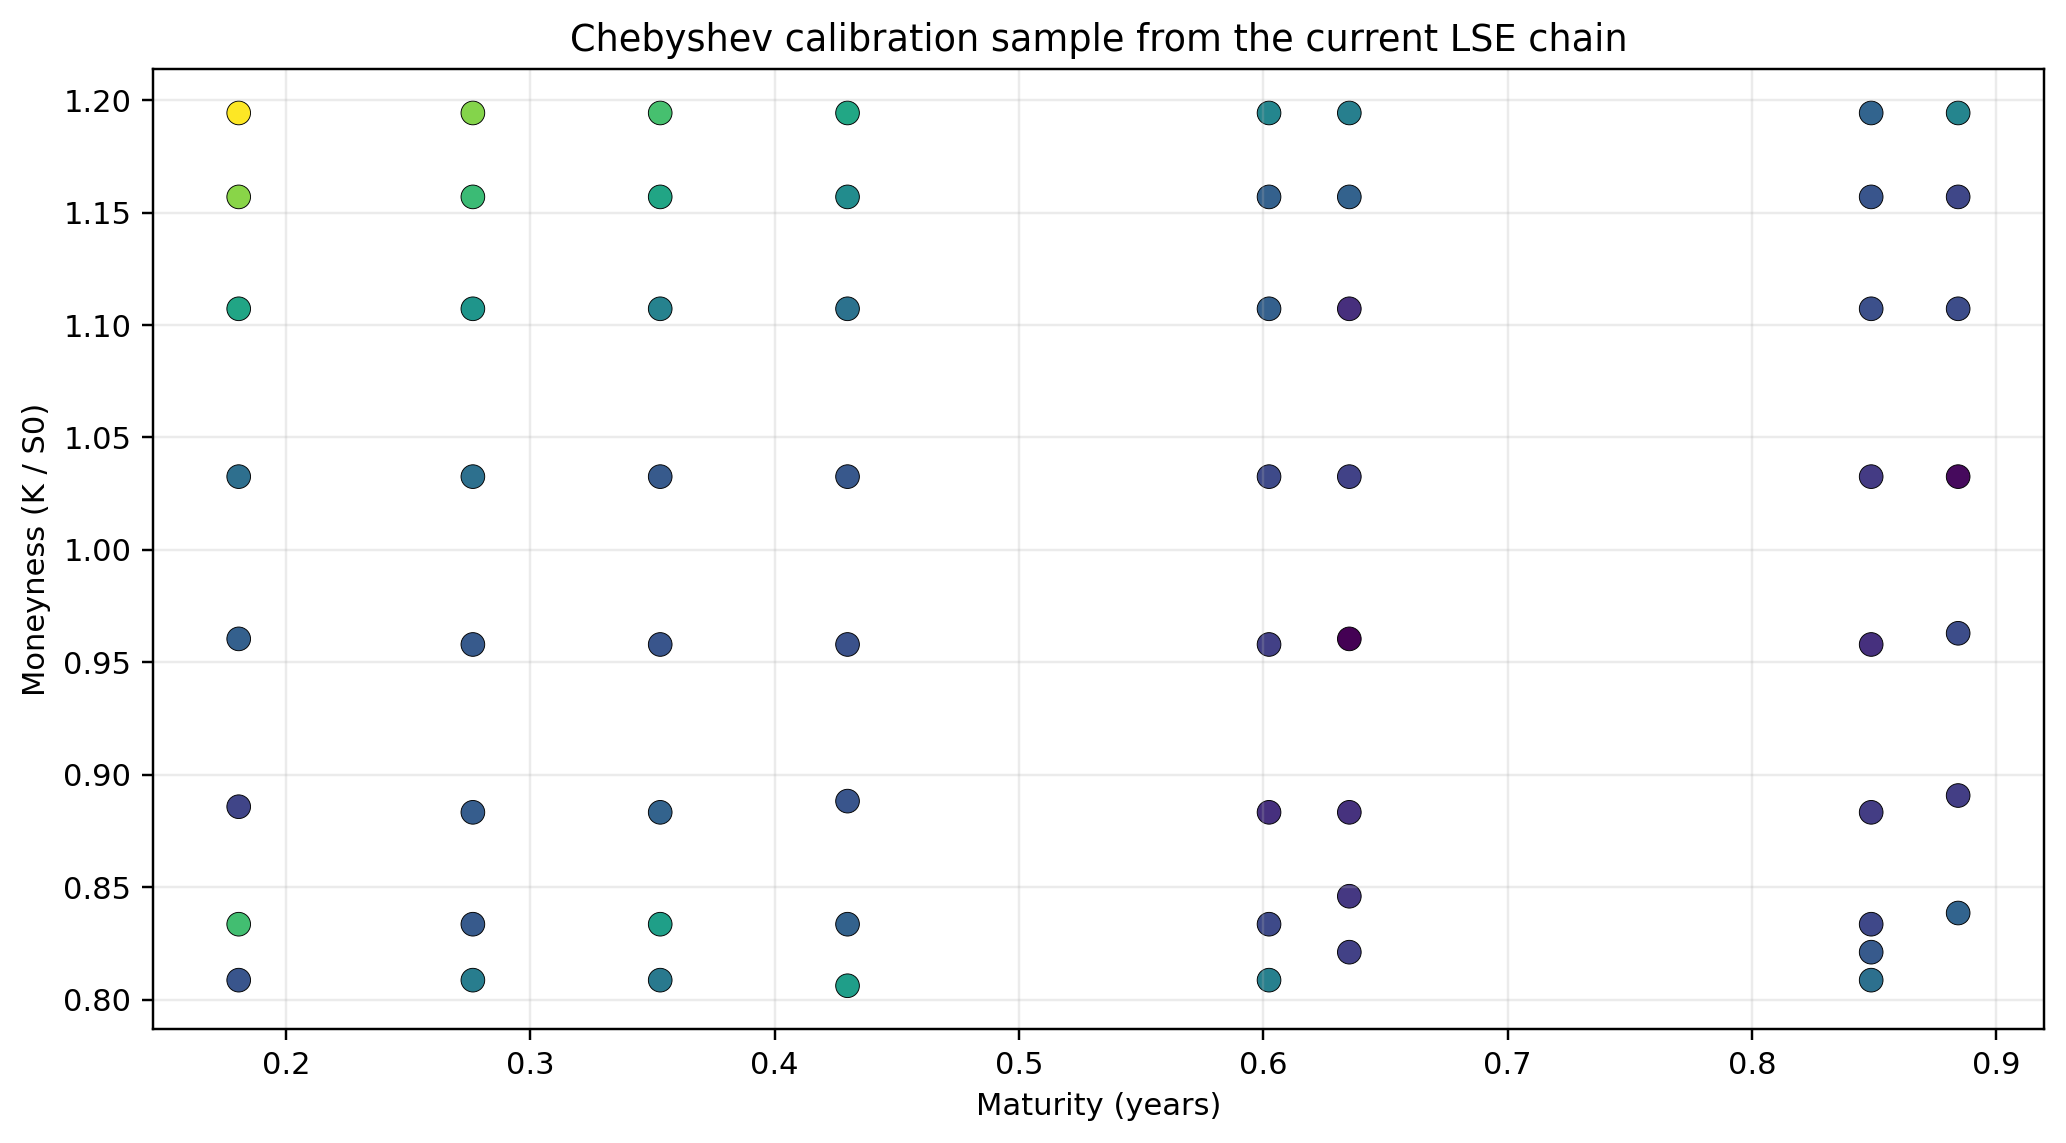
\includegraphics[width=0.95\columnwidth]{figures/sampling_comparison.png}
  \captionof{figure}{Final 2 September 2026 GLD surface and fixed CC64 geometry: 64 distinct actual contracts are selected from 605 eligible calls across 12 expiries and 146 strikes. Colour represents observed implied volatility.}
  \label{fig:chebyshev_audit}
\par}

\subsection{Why structured sampling is retained}
The option surface is irregular in strike and maturity. Team 8 therefore passes a fixed $8\times8$ Chebyshev--Chebyshev subset to the optimizer rather than allowing densely listed regions to dominate the loss. Every target is mapped to the nearest still-unused actual option: the 64-point calibration set contains no synthetic contracts. The figure audits the same 2 September parameter snapshot used by the refreshed valuation.

\begin{methodbox}[Evidence status]
The calibrated inputs, residual maps and valuation paths share the same 2 September Team 8 parameter set. The U.S. Treasury curve is dated 2 September as well; the separate Q2 realized-gold level anchor remains explicit in the valuation contract.
\end{methodbox}

\subsection{What the residual maps add}
The residual heatmaps show where each specification systematically over- or under-prices the observed implied-volatility surface. Black--Scholes leaves the strongest smile and term-structure pattern. On this snapshot Heston provides the lowest IV RMSE at 49.4881 bp; Full Bates--Hawkes follows at 52.9714 bp and Bates at 54.6273 bp. The fitted Hawkes branching ratio is 0.5569, below the stationarity boundary but economically material. The four maps are arranged as a two-by-two comparison so their common axes and colour scales remain directly comparable.

\end{multicols}

\vspace{4pt}
{\centering
\begin{minipage}[t]{0.485\textwidth}
  \centering
  
\includegraphics[width=\linewidth]{figures/black_scholes_residual_heatmap.png}
  \par\vspace{1pt}{\footnotesize\textbf{(a)} Black--Scholes\par}
\end{minipage}\hfill%
\begin{minipage}[t]{0.485\textwidth}
  \centering
  
\includegraphics[width=\linewidth]{figures/heston_residual_heatmap.png}
  \par\vspace{1pt}{\footnotesize\textbf{(b)} Heston\par}
\end{minipage}

\vspace{2pt}

\begin{minipage}[t]{0.485\textwidth}
  \centering
  
\includegraphics[width=\linewidth]{figures/bates_residual_heatmap.png}
  \par\vspace{1pt}{\footnotesize\textbf{(c)} Bates--Poisson\par}
\end{minipage}\hfill%
\begin{minipage}[t]{0.485\textwidth}
  \centering
  
\includegraphics[width=\linewidth]{figures/bates_hawkes_residual_heatmap.png}
  \par\vspace{1pt}{\footnotesize\textbf{(d)} Full Bates--Hawkes\par}
\end{minipage}
\captionof{figure}{Implied-volatility residual maps for the common 2 September CC64 sample. Blue denotes model IV above market IV and red denotes model IV below market; Heston records the lowest in-sample IV RMSE.}
\label{fig:residual_maps}
}
\vspace{4pt}

\begin{multicols}{2}
\raggedcolumns
